\documentclass[11pt]{article}
\author{Angus Blance}
\title{Agent Based Model For Civil Unrest}

%pacages
\usepackage{amssymb}
\usepackage{amsmath}
\usepackage{graphicx}
\usepackage{listings}
\usepackage{float}
\usepackage[round]{natbib}
\bibliographystyle{plainnat}

\linespread{1.6}

\usepackage{color} %red, green, blue, yellow, cyan, magenta, black, white
\definecolor{mygreen}{RGB}{28,172,0} % color values Red, Green, Blue
\definecolor{mylilas}{RGB}{170,55,241}


\begin{document}
	\maketitle
	\tableofcontents
	\newpage
	\section{Abstract}
	\section{Introduction}
	\textbf{Instances of large-scale disorder happen around the world regularly, resulting in significant damage to property and human life. Given the destructive nature of such events, finding means in which to mitigate the damage is necessary. In this report, we present an Epstein's agent-based model (ABM) that replicates the behaviour of civil unrest, and we demonstrate how the use of smoke by police forces can effectively reduce the number of participants in a riot.}
	
	\section*{What Causes A Riot}
	 Large scale disorder can be caused by many things such as deprivation, poor police relations, legitimacy of a government or just to many people in one area. Once a riot has started it then gets out of control very fast usually epidemic like(ref 2.). Factor's for this can be knowledge of an ongoing riot through social media or friends and rational choice theory as in if there are shops being looted and police are not doing anything you are more likely to join. Riots can then be continued if there is inadequate policing.\\
	 \\	
	 Modelling such events can be done in many ways and takes many disciplines, such as crowd dynamics, mathematics, Computer science and Psychology. In this report the model is based upon Mathematics and heavily uses computer programming to simulate our mathematical model. We also explore environmental criminology theory, which is the idea that someone is morel likely to join in the chaos if they can see or have knowledge of said chaos.
	
	\section{My Model}
	\subsection{What is an Agent Based Model}
	An agent-based model (ABM) is a computational modelling technique used to simulate the behaviour of individual agents and their interactions within a system. Each agent within the model has a set of rules which it obeys by, we then observe how these rules that our agent does affects itself and the other agents around it.\\
	\\
	For this study, I employ an ABM to simulate \citet{epstein2002modeling} Model for civil violence , which consists of three agents: quiet agents (Q) who are not participating in the riot, active agents (A) who are rioting, and police agents (C) who arrest actives. Each agent is placed on an N by N board\\
	\\
	Attributes for these agents are given:\\
	\\
	Quiet:\\
	-Qalk around the board at random\\
	-Calculates the amount of police and actives within its vicinity\\
	-Becomes active depending on number of Cs and As in vicinity\\
	\\
	Active:\\
	-Walk around randomly\\
	\\
	Police:\\
	-Walk around randomly\\
	-When near an active they arrest them and take them off the board\\
	\\
	
	\subsection{Mathematical Model}

	
	\subsection*{How Quiets Chose to Become Active}
	The main mathematical model that is now going to be shown is taken from \citet{epstein2002modeling} where we first find the Grievance given by
	\begin{equation}
		G = H(L-1)
	\end{equation}
	where H is the hardship of each specific non police agent and L is the legitimacy of the government which we set at the beginning of the model. \\
	\\
	Now we find the probability (p) to be arrested which each non police agent needs to calculate before they decide whether or not they wish to riot
	\begin{equation}
		P = 1 - EXP(-k(C/A)_{v})
	\end{equation}
	Note the subscript v notates the vision which each civilian has. C is the number of police in the vision v and A is the number of rioters in vision v. The civilian counts himself when counting A as he wants to see how the riot would be once he is added. K is just a constant which we set such that P = 0,9 when C=A=1, so k = -ln(0.1). \\
	\\
	For an example, We look to Figure 1 where we have our green dot as our quiet, the red dots are our actives, the blue dots are our police and the black box represents its vision v of our green quiet in the middle. For this example the vision of our agent is 1. We have 2 police and 2 actives within our agents vision.\\
	\begin{figure}[H]
		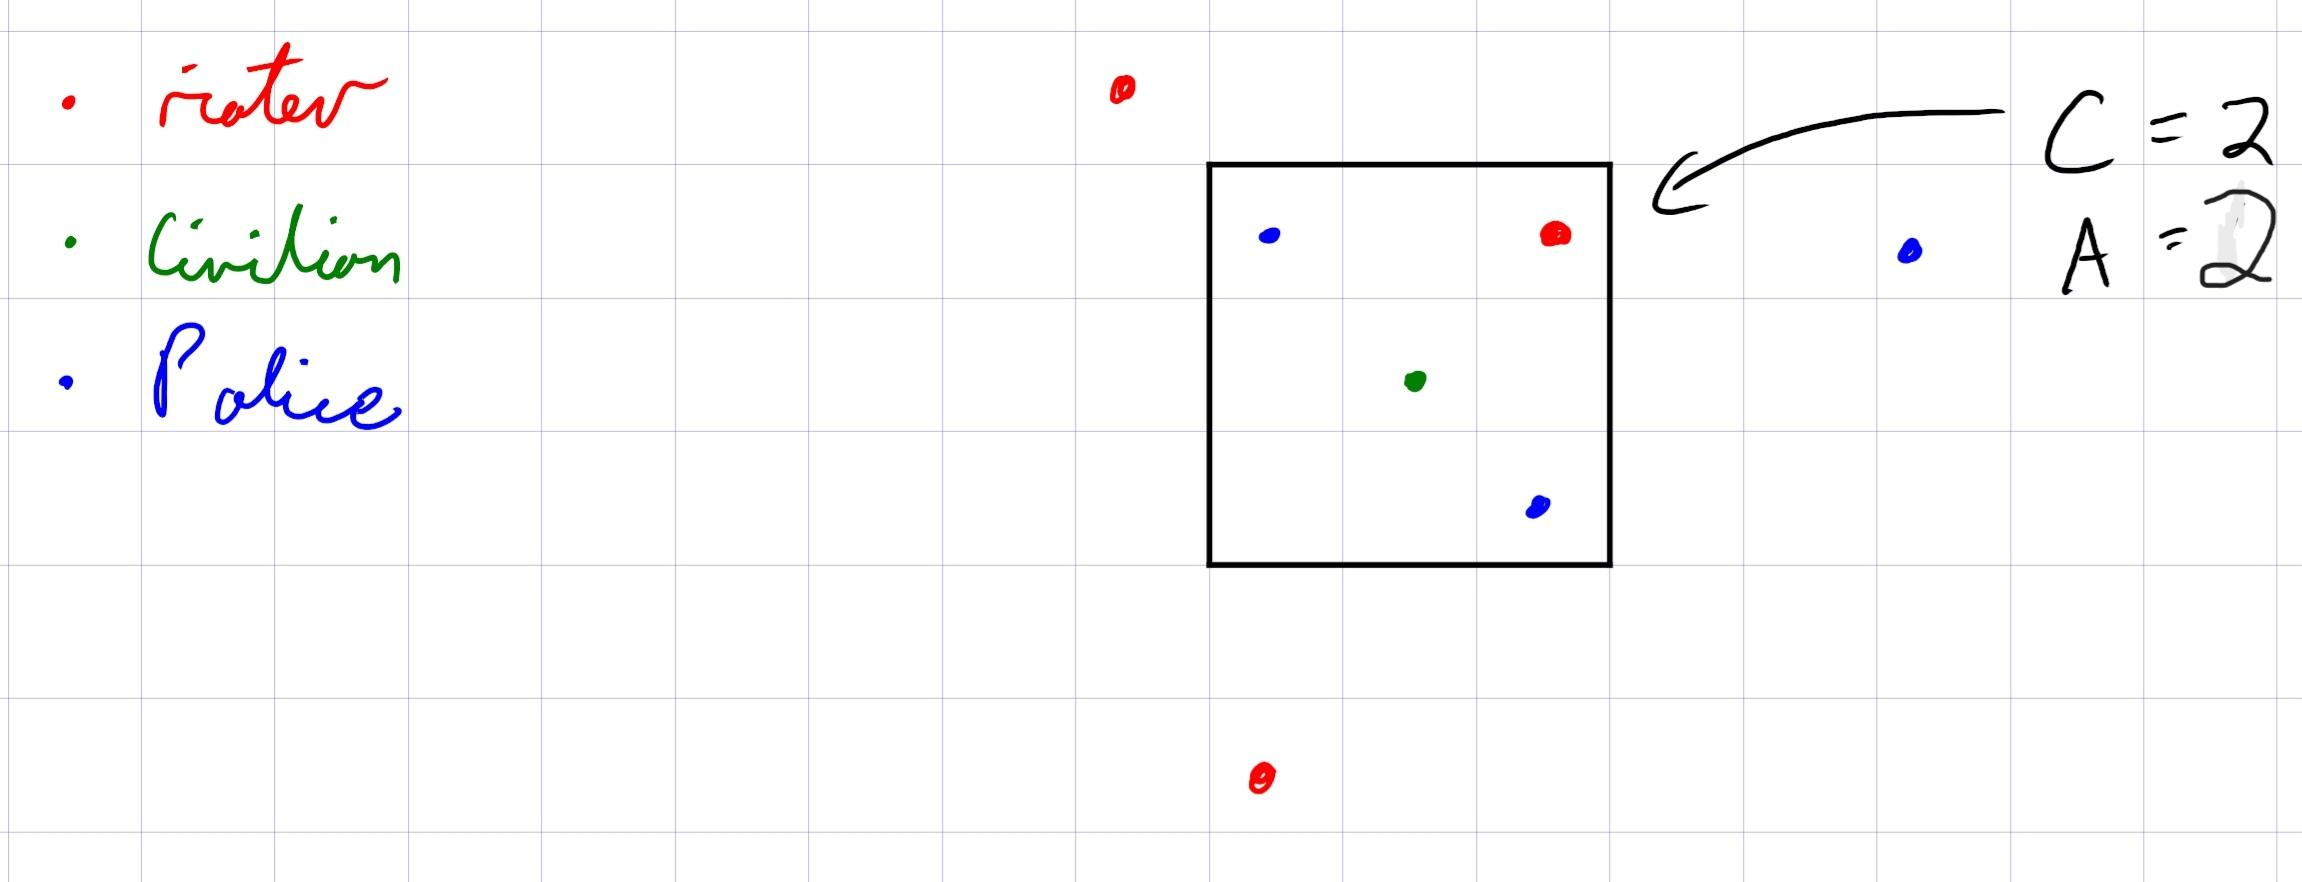
\includegraphics[width=\linewidth]{vision example.png}
		\caption{vision example}
		\label{fig:boat1}
	\end{figure}
	
	from this we can now define the net risk $N = RPJ$ where J is the maximum jail time one faces once he has been caught by a police officer. The max jail time is set before the model is run to whatever jail time is deemed fit and the amount of time someone will spend in jail is given from U(0,max jail time).\\
	we now  have all we need to create the agent rule:\\
	\begin{equation}
		Agent \; rule: if \; G-N>T \; riot; \; otherwise \; stay \; a \;  civilian
	\end{equation}
	so the difference in G and N is the expected utility of expressing ones private grievance whilst T is the utility of not.
	
	
	

	
	\newpage
	\section{Computational Approach and Implementation}
	
	First of all we have our N $\times$ N board say N=10 we the have figure 2\\
	\\
	\begin{figure}[H]
		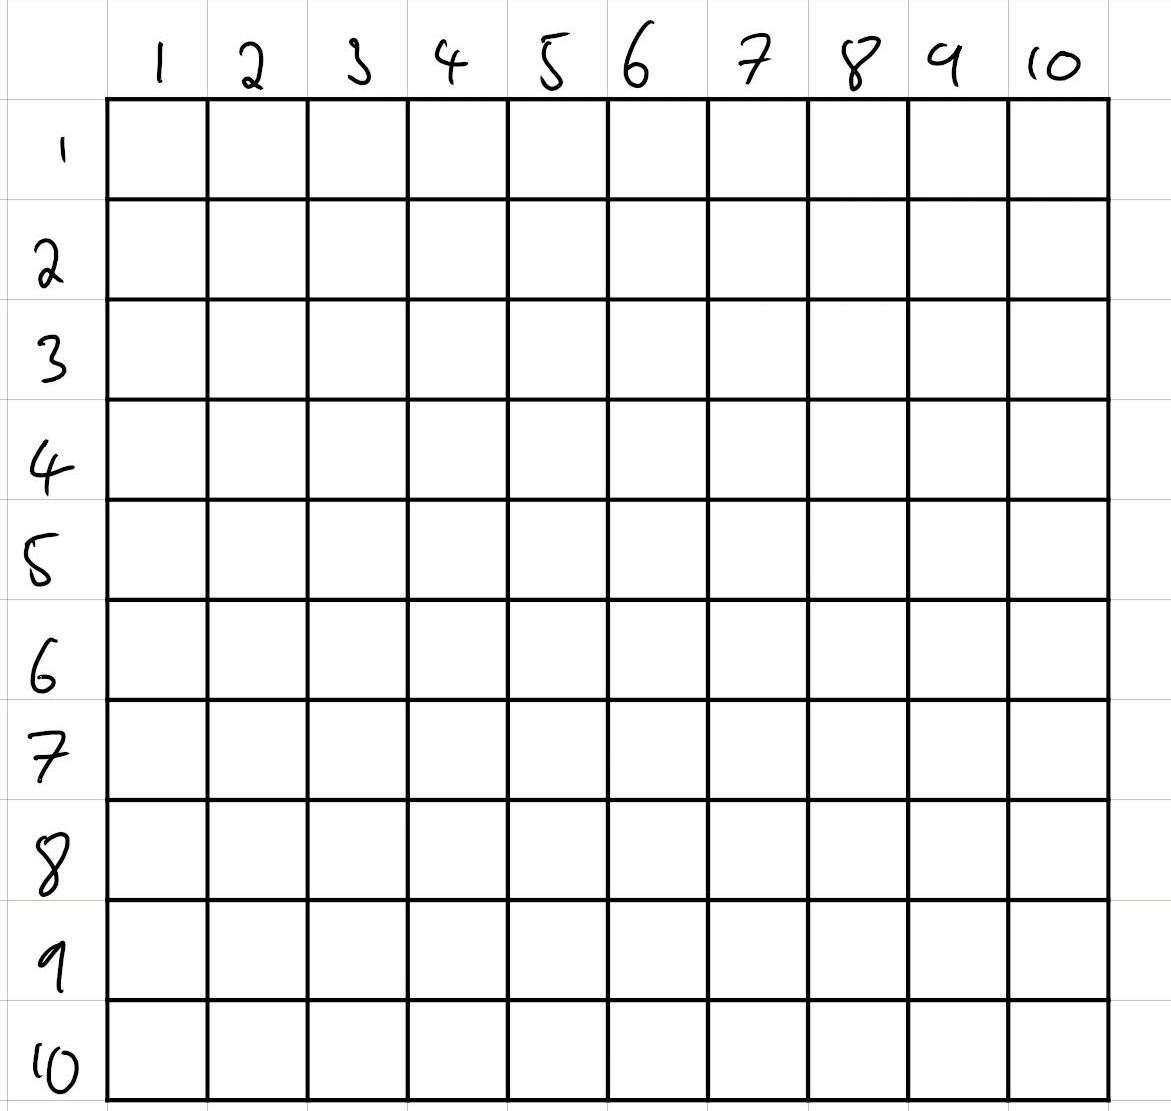
\includegraphics[width=\linewidth]{Visual Grid.png}
		\caption{Grid}
		\label{fig:frenchriot}
	\end{figure}
	Now agents are introduce to the model with attributes as described prior, the Actives are denoted by the colour red, our quiets  green and our police Blue. Say we loop through our hole N $\times$ N grid and place 20 quiets and 10 police at random we will end up with something like Figure 3\\
	\begin{figure}[H]
		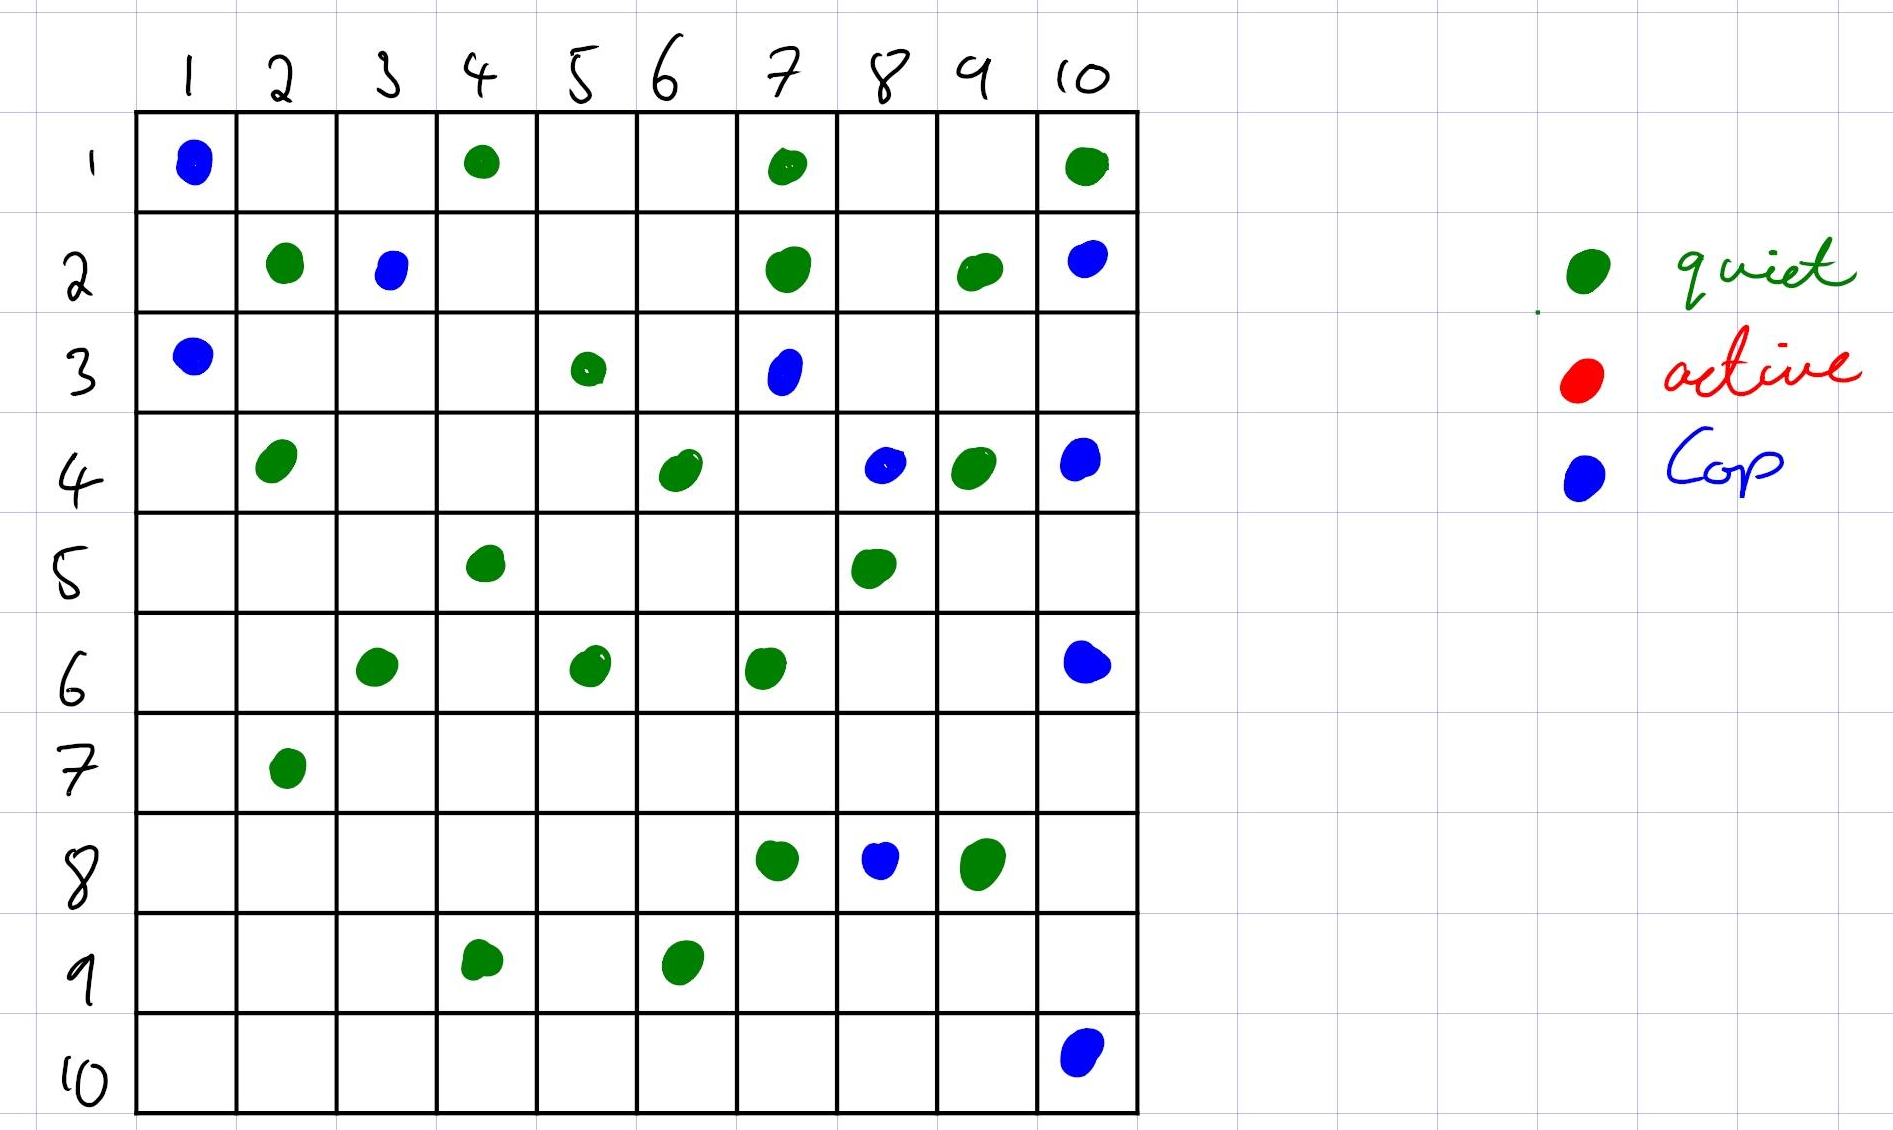
\includegraphics[width=\linewidth]{cops and quiets on grid visual.png}
		\caption{Grid with Agents}
		\label{fig:frenchriot}
	\end{figure}
	Great! That's our hole grid set up. But also note that each individual quiet has 2 attributes to them (risk level and Hardship) which is easier to see on a 10 $\times$ 10 example run on our code in Matlab as shown in figure 4\\
	\begin{figure}[H]
		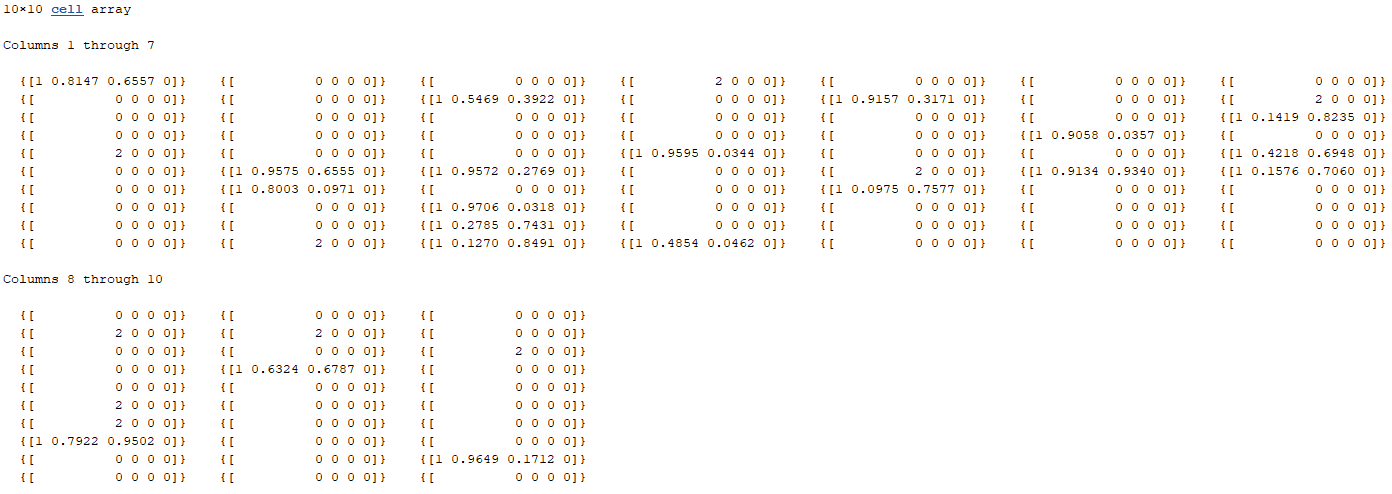
\includegraphics[width=\linewidth]{Matlab 10 by 10 matrix example.png}
		\caption{Grid on Matlab}
		\label{fig:frenchriot}
	\end{figure}
	Notice how our model stores the risk level and Hardship by making our board a cell array and storing multiple values for each cell. Also see how all of the cops have no hardships or risk, This is because they do not have the attribute to become an active meaning giving them such values will be redundant.\\
	\\
	\subsection{Moving}
In the model every agent will only move one space (Cell) at a time how they move is shown in figure 5  where the arrows on the diagram on the left show the direction in which each agent will move and the diagram on the left shows the grid after each person has moved\\
	\\
	\begin{figure}[H]
		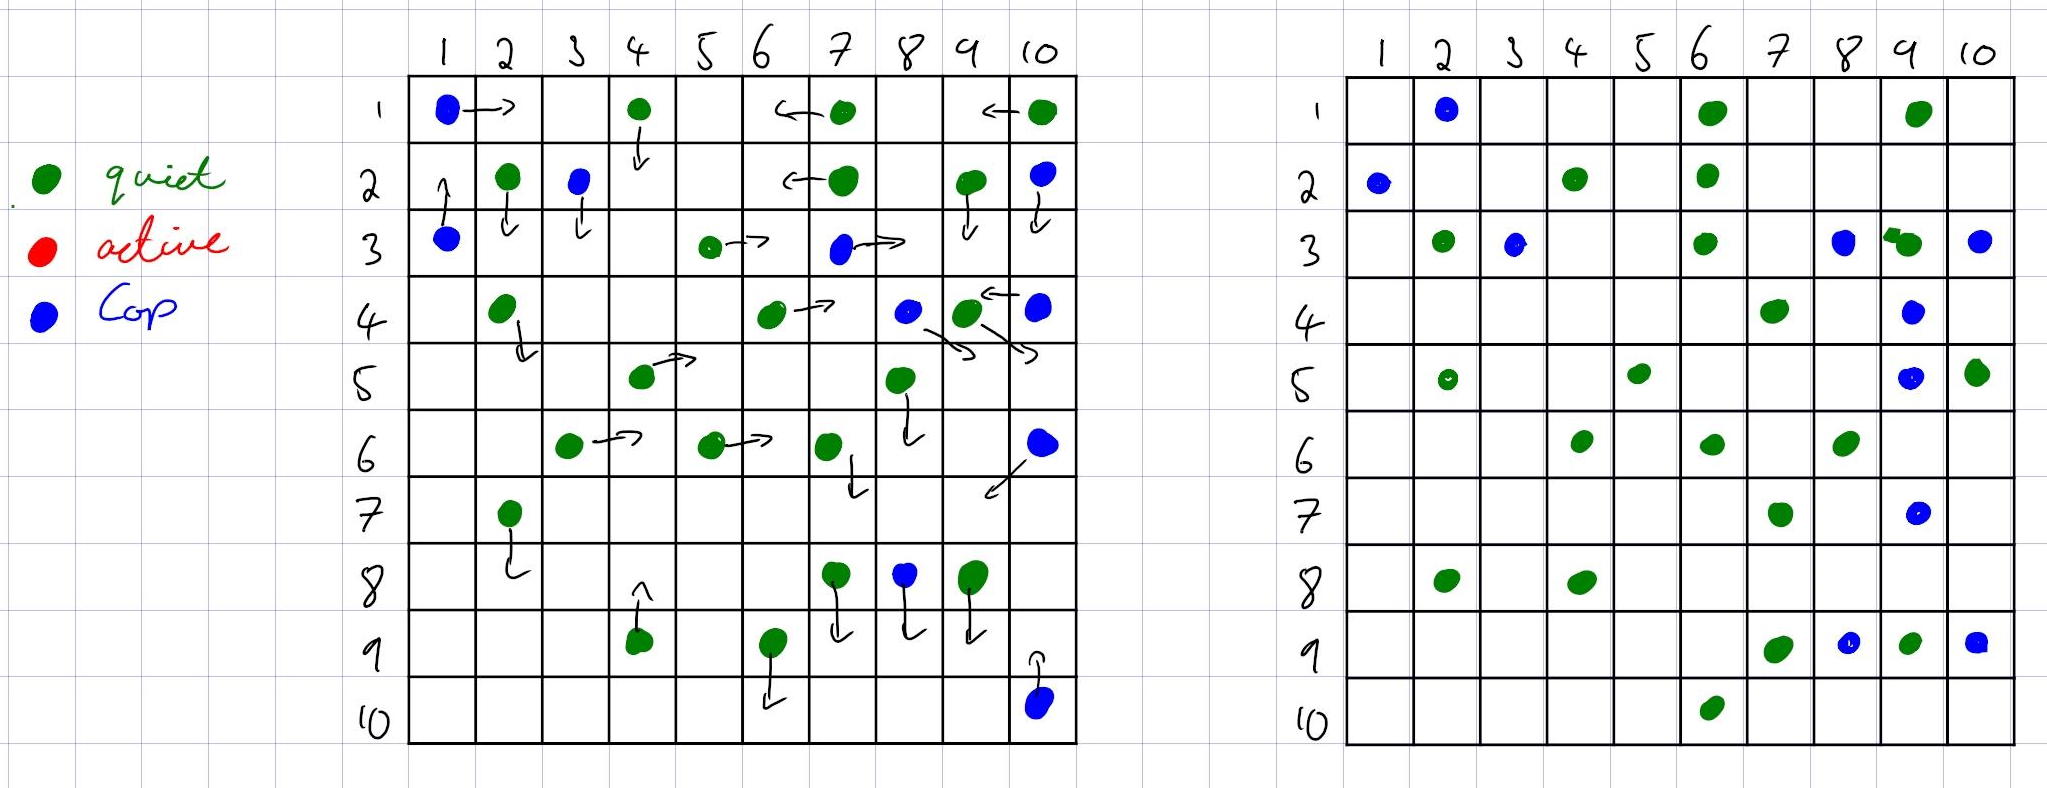
\includegraphics[width=\linewidth]{Movement visual.png}
		\caption{French riot}
		\label{fig:frenchriot}
	\end{figure}
	see how the police in column 10 row 4 (10,4) moves to space (9,4) which is already occupied by a quiet? This happens due to how the model loops through the grid. This is done from the top left of the grid to the bottom right (like a book) meaning that the quiet in space (9,4) has already moved to (10,5) before the police makes his move into the space the quiet was just in.
	\\
	\\
	\subsection{Quiets and Actives The Descension to Riot}
	Just as before our model loops though the hole board, first starting form the top left and ending up on the bottom right. Whenever we land on a quiet we take its risk and hardship as well as searching in a M $\times$  M grid around said quiet to collect the number of A's and P's within its vision, as shown in the mathematical model.\\
	\\
	To explore this further lets take figure 6 as an example
	\begin{figure}[H]
		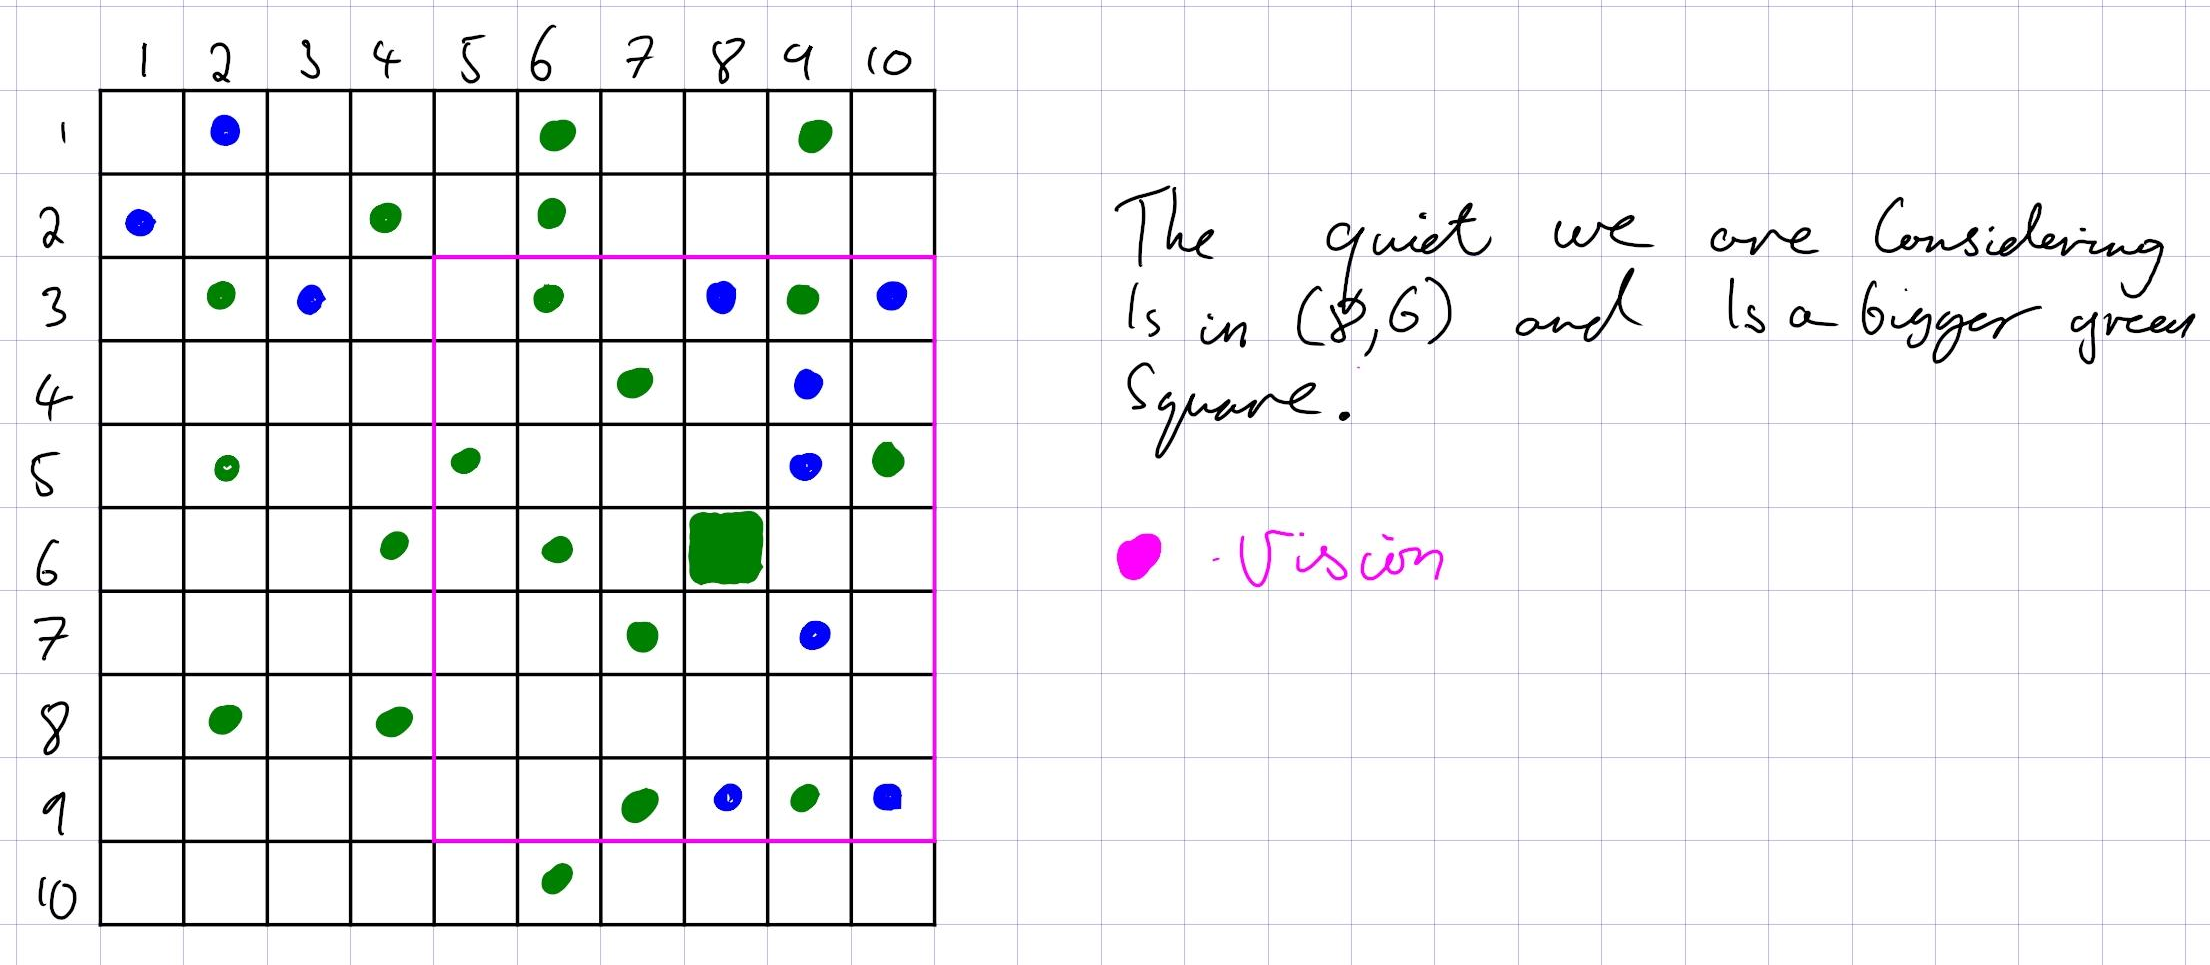
\includegraphics[width=\linewidth]{vision for single case.png}
		\caption{Vision Example for Single Case}
		\label{fig:frenchriot}
	\end{figure}	
	B
	Now looking at what data we have for our particular case in (figure 6) we have C = 7 and Q = 9 not including the quiet we are currently considering. \\
	\\
	For this particular	quiet to become active we need our agent rule to be satisfied. for this we want N to be small so that the left hand side is greater than the right hand side, looking at N
	\\
	\begin{equation}
			N = RPJ 
	\end{equation}
	Where R is the level of risk aversion they will take given to each non police agent, higher level of risk aversion the less likely they are to take risks. We can see that if R increases N will clearly increase as well making the agent less likely to become active. Just as increasing R makes an agent less likely to riot, using the same logic we can see that decreasing R makes an agent more likely to riot.\\
	\\
	Now looking at P the other factor in calculating N
	\begin{equation}
		P = 1 - EXP(-k(C/A)_{v})
	\end{equation}
	We have C and A from figure 6 which we sub into (5) to get get P = 0.9999999 for our specific case, which makes sense as there are no A's within the vicinity of our Q and there are many C's meaning the probability of arrest should be high. Also see that as C $-> \infty$ P $-> 1$ (less likely to become active) and as A $-> \infty$ P $-> 0$ (more likely to become active). looking at (4) again we can see that greater P values creates a greater N value making our agent less likely to become active, the more likely someone is to be arrested the less likely they will become active\\
	\\
	say in our particular case J = 5 which is a smallish jail sentence which should mean a rioter is more likely to riot then our N = R$\times$4.9999995 and using this and substituting G from (1) we obtain
	\begin{equation}
		G-N = H(L-1)-R \times 4.9999995
	\end{equation}
	Say we want our Q to become active we want (6) to be Large such that it is $>$ T meaning we want H(L-1) the total grievance of this agent to be large and R $\times$ 4.9999995 to be small. First for H(L-1) to be large we need want the hardship of our specific individual to be large and the legitimacy of our government to be low, Note that just having a high level of hardship does not mean our Q will become A, we need both a high hardship AS WELL as a low perceived legitimacy of the government.\\
	\\
	\subsection{Police Arresting}
	C's move just the same way as the Q's and A's, However they cannot become A. The main characteristics C's have is the ability to arrest this is done by them just happening to walking about and searching similarly to Q's and A's "scanning" the area around them. If an A is within a C's vision it then arrests them putting them into "jail". The jail is a matrix storing all actives that have been caught by police. What an arrest would look like in my model can be shown in figure 7 where on the left a C is next to an A and in the next the A has been put into jail. The jail sentence J is set to 5 in this example meaning it takes 5 iterations for our agents to be set free from our jail. The Jail inmate's number next to him is the time he has spent in jail which goes down by 1 after the turn has taken place
	\begin{figure}[H]
		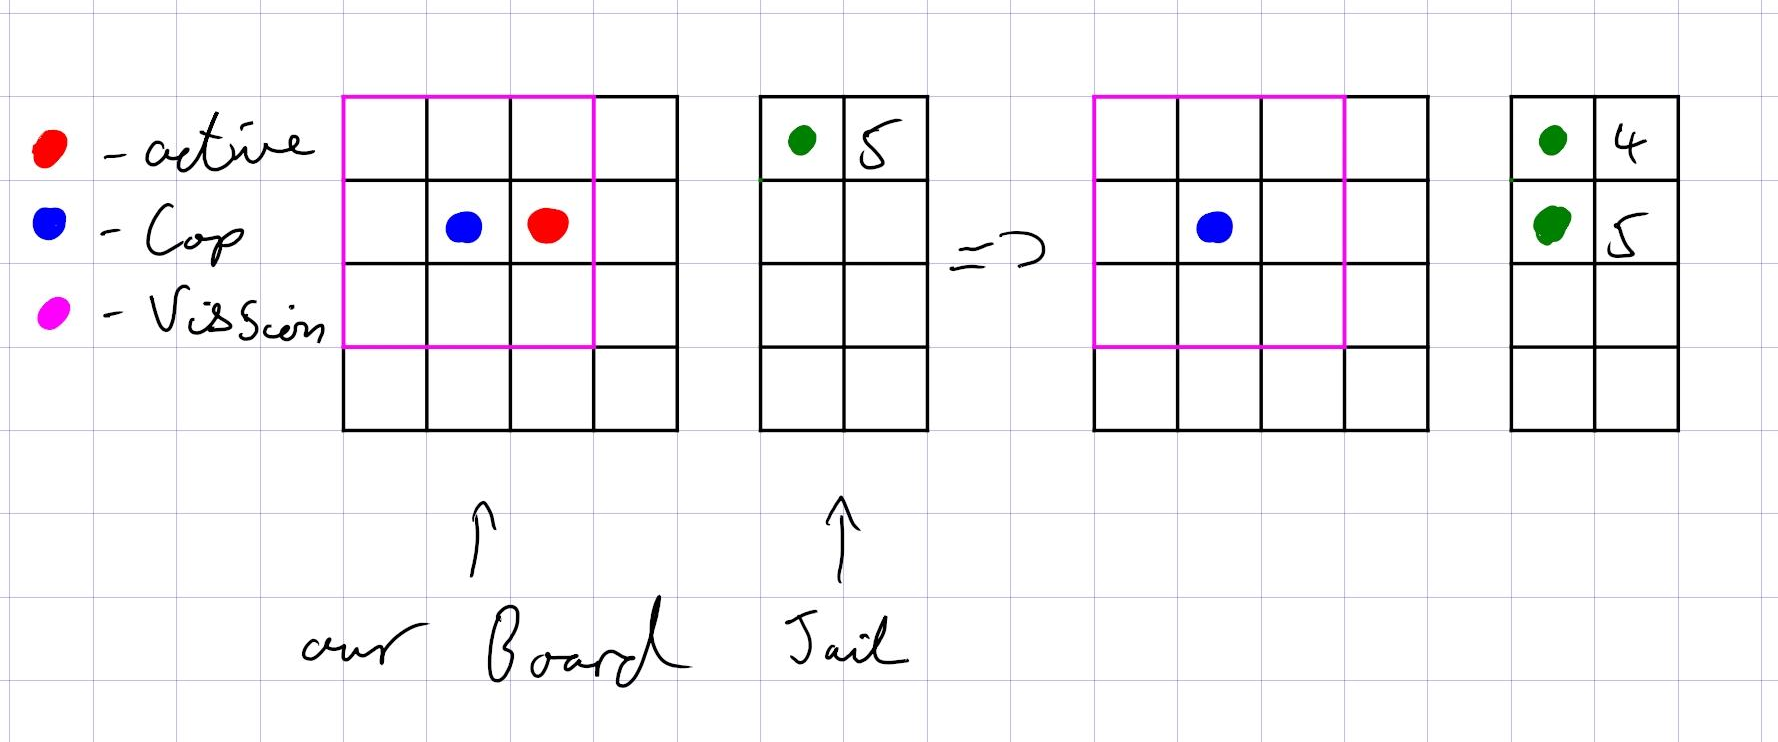
\includegraphics[width=\linewidth]{arresting visual.png}
		\caption{Arresting Example}
		\label{fig:frenchriot}
	\end{figure}	
	\subsection{Smoke}
	For my smoke a created another empty N $\times$ N array same as figure 4. But for this one each cell has 2 values the first being a 1 or a 0 representing if the square is occupied by smoke or no smoke respectively. A simple example of this is seen in figure 8 where the blue C sees an A within its pink vision. It then promptly throws smoke at the A
		
	\begin{figure}[H]
		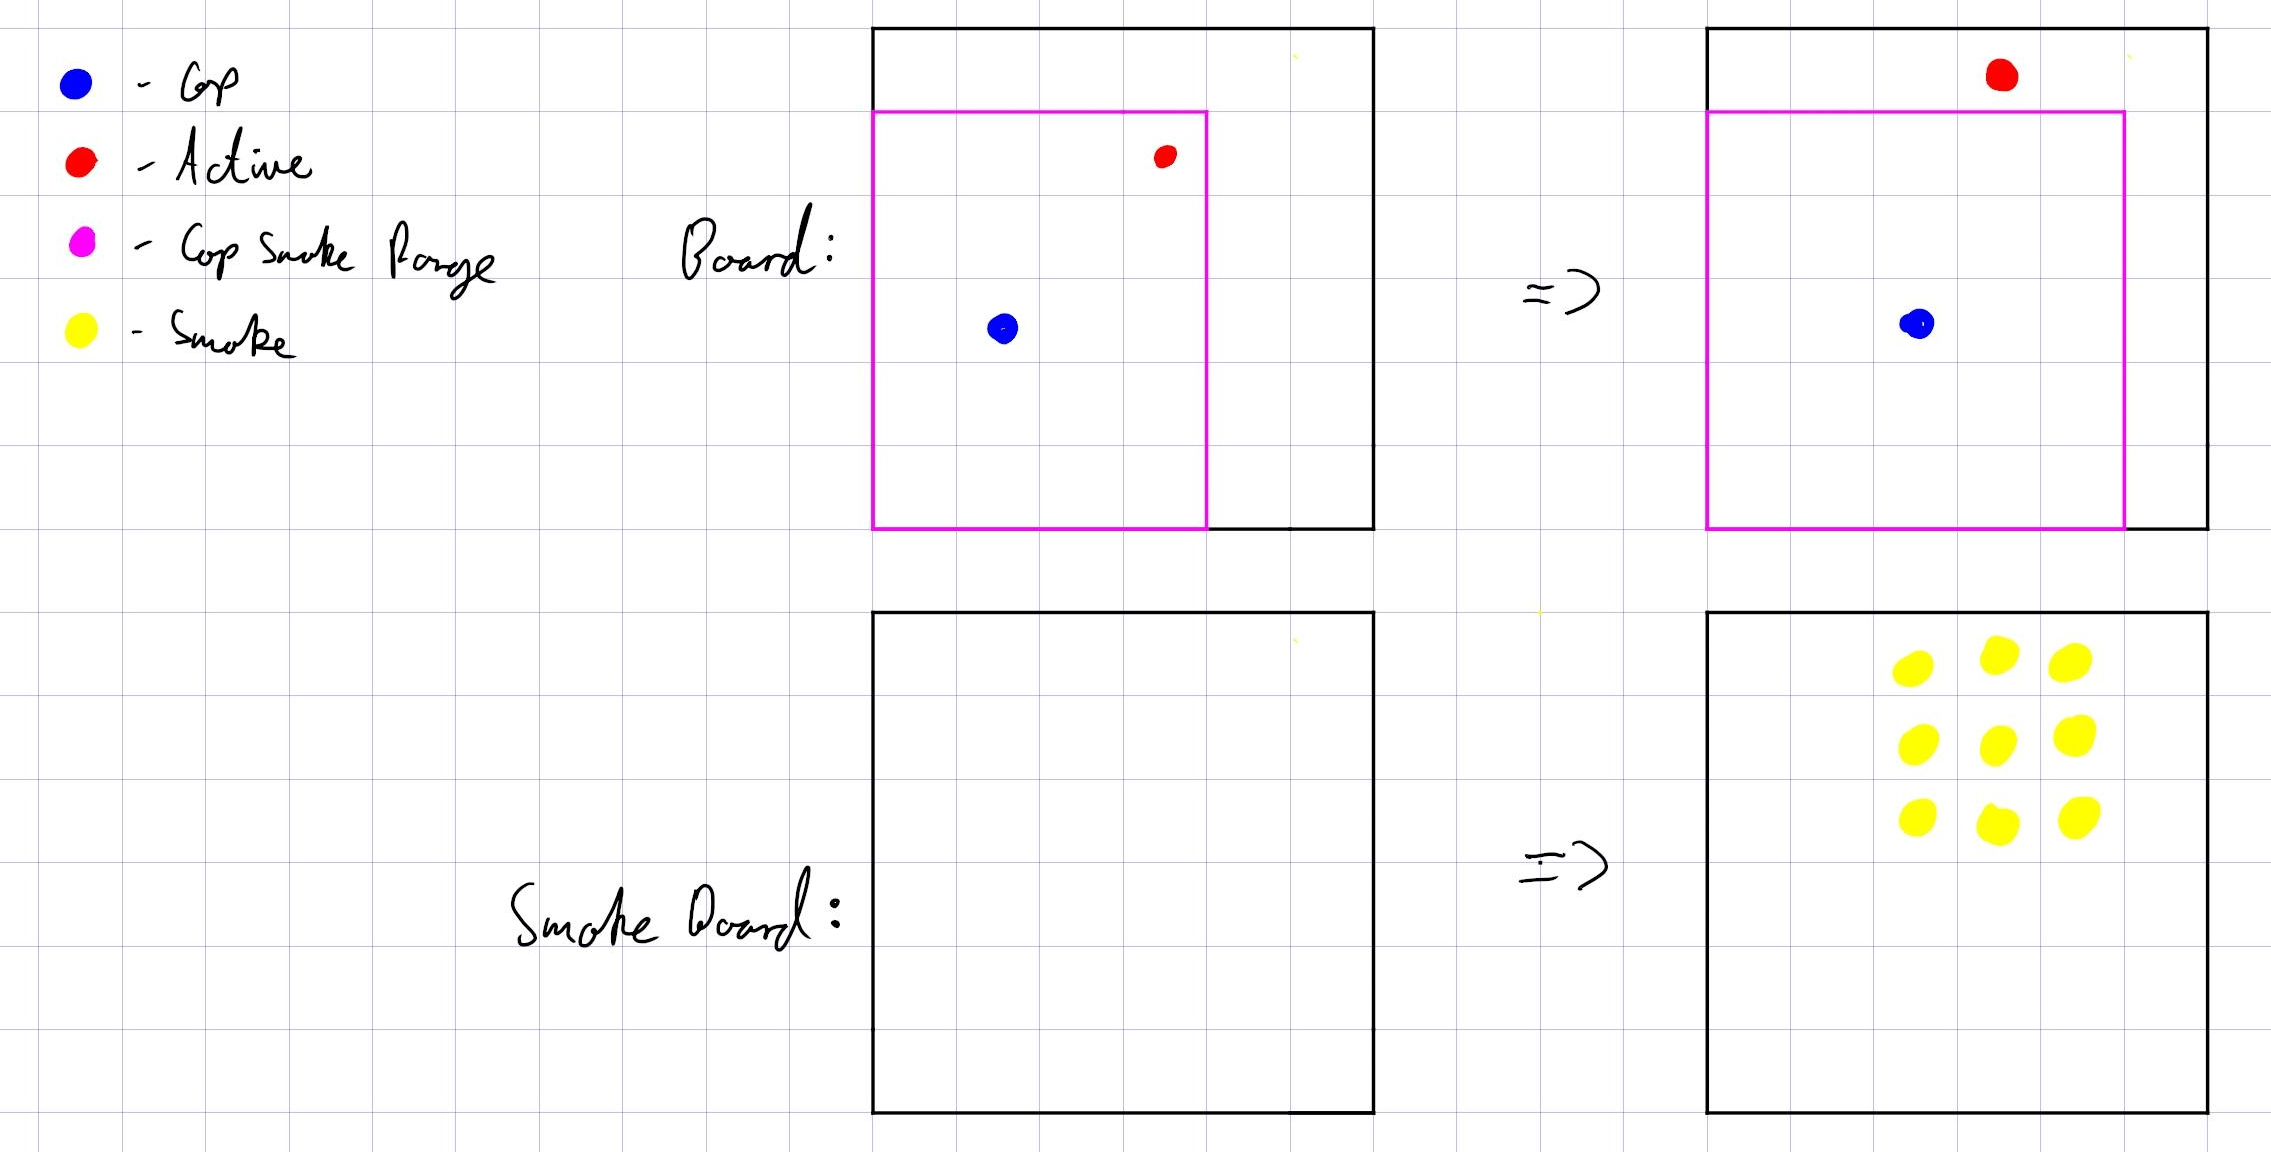
\includegraphics[width=\linewidth]{smoke visual.png}
		\caption{French riot}
		\label{fig:frenchriot}
	\end{figure}	

	
	\newpage
	\section{Results From my Model 1}
	In this section I run my model but change the variables of the model such as the C/A density, the vision of agents and the perceived legitimacy to see if I find any trends. sections 5.1 up to 5.4 are nearly identical to the results of Epstein's model showing that my model works as intended. 5.5 and 5.6 are not on any paper that I have found.\\
	\\
	Each iteration of my model consists of:\\
	1 - all agents moving, \\
	2 - non police agents deciding whether or not to riot\\
	3 - police agents arresting one active within its vision
	
	\subsection{Deceptive Behaviour}
	This is the case where a quiet is green when C are not near by but when cops leave the area they become active. This is due to the C/A ratio changing. As in when a C is near by the probability of arrest increases making G-N smaller. If smaller than T then they turn Q. The same applies for if a cop leaves there vision that they have a higher chance to become active.\\
	\\
	Epstein compares this behaviour to Mao Zedong's directive where revolutionary's must "swim like fish in the sea" describing how revolutionary's must hide in the crowd and not distinguish themselves from the quiets waiting for the right time to start a revolution.
	
	\subsection{Snowball Effect}
	If a small group of quiets go active then this can lead to even more quiets going active, we observe this in figure 10 where area's where there is a low density in cops leads to quiet's becoming active, which in turn decreases the C/A ratio giving a lesser probability of arrest meaning even people with a high level of risk aversion have a higher chance of joining in the riot on the next iteration.
	\begin{figure}[H]
		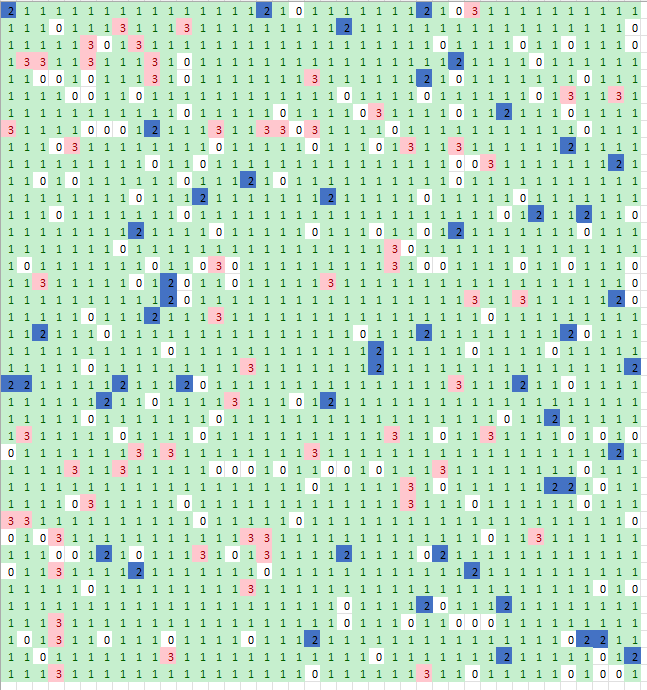
\includegraphics[width=\linewidth]{snowball_1_T0.1.png}
		\caption{C=1400,Q=50,V=2,T = 0.1, L=0.89}
		\label{fig:}
	\end{figure}
	This can be illustrated even further by decreasing our T value shown in figure 11.\\
	To be the first to riot you have to have a very low risk aversion or very high hardship. But the more people that join the riot the lower the probability of arrest is and the risk involved is much lower.
	\begin{figure}[H]
		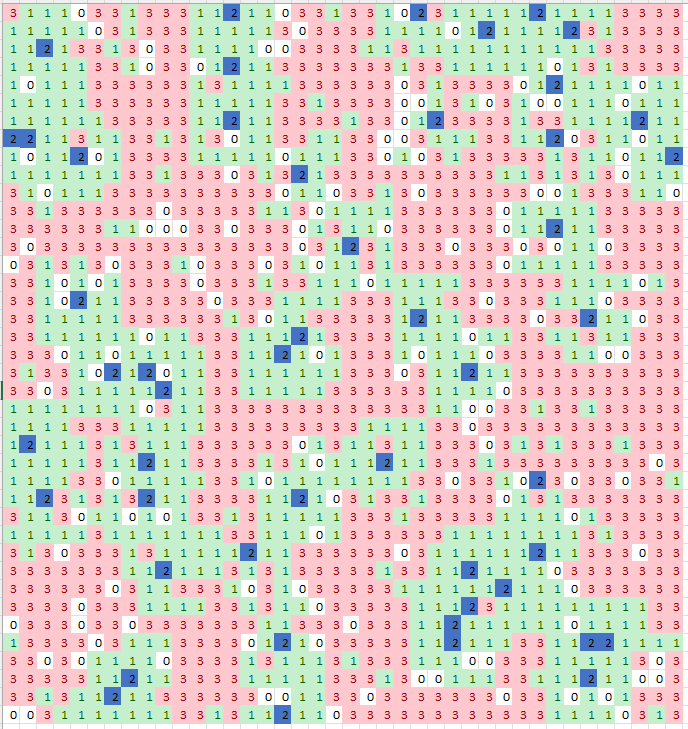
\includegraphics[width=\linewidth]{snowball_2.png}
		\caption{C=1400,Q=50,V=2,T = 0.01, L=0.89}
		\label{fig:}
	\end{figure}

	\subsection{Effect of Legitimacy}
	Initial conditions: C = 118, Q = 1120, v = 6(all agents), T = 0.1\\
	\\
	
	To explore the effect of legitimacy the model is run the model starting with L = 0.9 and decreasing our legitimacy by 0.01 each iteration of the model. Looking at figure 12 We see the yellow legitimacy line is straight and constantly decreasing, the number of rioters is horizontal running all the way along the x-axis so the number of rioters = 0 at every iteration and the number of prisoners steadily increases throughout. The number of rioters is never above 1 this is because a small decrease in legitimacy only makes a few quiets want to come active and the get arrested straight away not allowing the snowball effect to take place.
	
	\begin{figure}[H]
		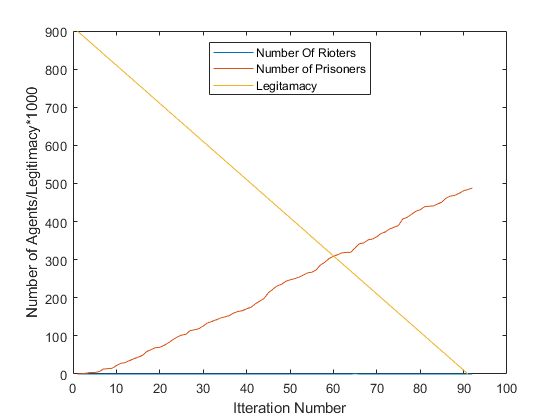
\includegraphics[width=\linewidth]{effect of Legitamacy reduction.png}
		\caption{Slow Decrease in Legitimacy}
		\label{fig:yu}
	\end{figure}
	Now (figure 13) instead of a slow decrease in legitimacy over time we have a constant high L = 0.9 for 77 iterations and then a sudden drop to L =  0.7  for a further  43 iterations. There is stark difference between the figures 12 and 13. 15 has a massive outburst in actives revolting against the government they are in with a significantly smaller change in legitimacy.\\
	
	\begin{figure}[H]
		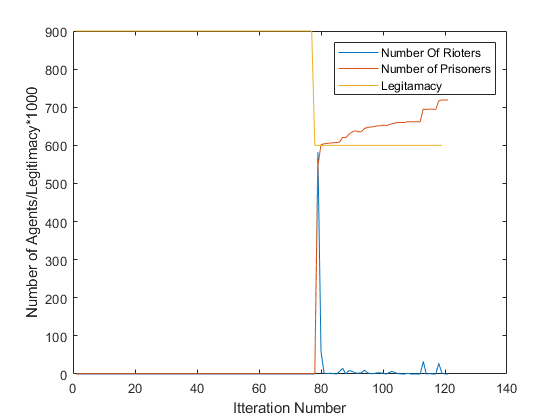
\includegraphics[width=\linewidth]{sudden effect of Legitamacy reduction.png}
		\caption{Effect of a Sudden Drop in Legitimacy}
		\label{fig:frenchriot}
	\end{figure}
	
	The reason that figure 15 has a sudden revolt is due to the sudden decrease in L creating a larger amount of active which depress local C/A ratios which mean that in the next iteration not only will they have a lower L but also the lower C/A making the likelihood for one agent to riot much greater (snowball effect)\\
	\\
	This result gives insight in tack-ticks which can be used for somebody to create a revolution. It shows that slowly releasing negative information from a government will not cause a riot or any real change. However releasing large amounts of negative information about a government at one time will create an even greater impact, even if the value of legitimacy the government decreases by a smaller amount than the total decrease in legitimacy in the slower method. Also note that releasing information is not the only way to lower legitimacy.\\
	\\
	Epstein compared this effect to a few real life situation's such as Mao Zedong who would isolate himself himself in the mountains for a big reappearance. Or even the return of leaders such as Vladimir Lenin and Ruhollah Khomeini after being exiled would come back with a big bang. Possibly this could even represent "triggering events" where the legitimacy of a government suddenly drops for instance an assassination.
	
	\subsection{Police Reductions}
	Initial conditions: C = 118, Q = 1120, v = 6(all agents), T = 0.1, L = 0.86, \\
	\\
	It would be though under an oppressive regime where there are loads of police enforcing the regime on their citizens that decreasing the oppressiveness by taking away police could result in a happier population. However as our model depicts in figure 16 we see that the people wait around as the government reduce the number of police until there seems like there are too few police to resist. This is very different to the gradual decrease in legitimacy shown above. In fact the small revolution that breaks out in figure 16 closely resembles a sudden decrease in legitimacy. This shows that for the model, the perceived legitimacy of the government is fundamentally different to the density of police in the model
	\begin{figure}[H]
		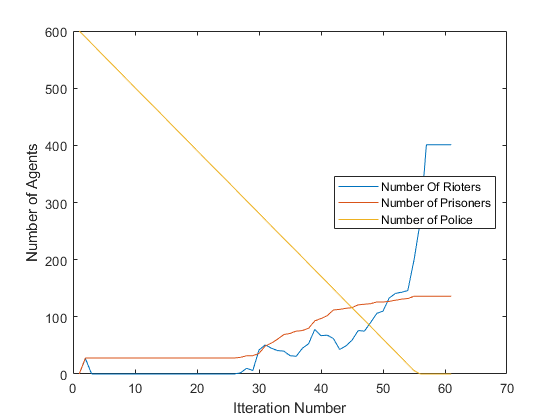
\includegraphics[width=\linewidth]{Police Reductions.png}
		\caption{C=600,Q=800,v=2,L=0.4,T=0.1}
		\label{fig:frenchriot}
	\end{figure}
	\citet{epstein2002modeling} compares what we see in the model to the French Russian and Iranian revolutions.
	\subsection{Simulating a 'Riot'}
	For my model I will simulate some sort of riot by placing all of my non police agents on one side of the board being the riot, and then the police on the other side of the board shown in figure 17
	\begin{figure}[H]
		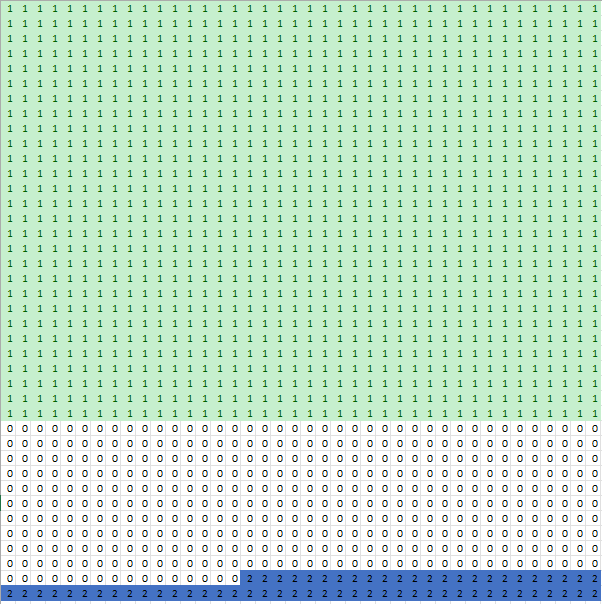
\includegraphics[width=\linewidth]{Riot Layout.png}
		\caption{C=64,Q=1120,v=2,T=0.1,L=0.82}
		\label{fig:frenchriot}
	\end{figure}
	The model is then run with this initial layout until there are no actives left. The jail sentence is set to be infinite, as usually when somebody is detained from a riot they don't get back into the riot. The other initial conditions we have are C=64, Q=1120, vision = 6 (police and non police), T=0.1, L=0.82\\
	\\
	from this new setup we get the results in figure 18 where we have the blue line showing how the number of rioters starting out in a "riot" formation decreases with time. We also have a red line across the x axis showing the number of rioters for random placement which we did in our previous examples. We then have the purple line showing the number of people removed from the "riot" as well as the yellow line showing the same but for the random placement.\\
	\\
	We can clearly see that when we place our agents in a riot formation they start of with a far greater number of actives due to a very low C/A ratio as there are no police whatsoever in the riot crowd. we then see that it takes far longer for the number of rioters in our riot to reach 0. We also see a far greater total number of non police agents going into jail when they are randomly distributed throughout the grid.\\
	\\
	This is a great example of how with correct policing and spacial awareness can affect whether or not a riot will get out of hand.
	
	\begin{figure}[H]
		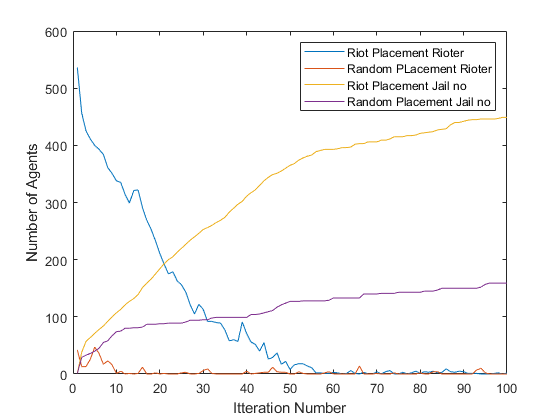
\includegraphics[width=\linewidth]{Riot Placement vs Random Placement.png}
		\caption{Riot Placement Vs Random Placement}
		\label{fig:frenchriot}
	\end{figure}
	
	\subsection{The Effect of Smoke}
	Initial Conditions: C = 118, Q = 1120, v = 6(all agents), T = 0.1, L = 0.86, smoke size = 6 (7 $\times$ 7 grid), smoke duration = 40, jail length = infinite \\
	\\
	First of all we simulate the exact same riot as we simulated before, except now we introduce our concept of smoke, from this we get figure 17\\
	\\
	\begin{figure}[H]
		\includegraphics[width=\linewidth]{smoke on a riot.png}
		\caption{The Riot Layout}
		\label{fig:frenchriot}
	\end{figure}
	from the figure we see that with and without smoke both start at about the same number of initial rioters. However looking at further iterations shows how the use of smoke Helps subdue our riot and makes the riot come to a halt at about 30 iterations. Whilst on the other had the model without the smoke takes a total of about 60 iterations to come to a halt! this is a big jump in the length of time in which it takes for the riot to stop, just by introducing smoke.\\
	\\

	\newpage
	
	\subsection{Model Analysis}
	Despite this model being pretty basic, it still manages to produce very interesting results which can be compared historical real world events. We managed to observe individual deceptive behaviour in which agents pretend to not be rebellious whilst they wait for the best time to strike as well how legitimacy and the density of police effects A's\\
	\\
	The main concepts that we observe in our model are described as "tipping points" by episteme (ref), these are moments in a regime when a large amount of people rebel and start a riot or even a revolution. We see a few such tipping points firstly from the snowball effect where we see that time is of the essence for a government to suppress a few active agents before more and more join them.  We then see our second tipping point occur when there is a sudden drop in perceived legitimacy causing a large outburst in active agents rebelling against their government. Our final tipping point is found when we slowly decrease the amount of police of an oppressive scheme where agents are being deceptive the hole time until they see an opportunity when there are far fewer police about to stop them.\\
	\\ 
	Along with these observations we then created a riot and saw how the effect of obscuring vision can affect how quickly a riot can be stopped!
	
	\section{Ethnic group model}
	Now I create the second model from the Epstein paper where we introduce two ethnic groups, a purple group and a green group. A few changes are made but the mathematical model is much the same for this, however now when one person from one group becomes active they will now take an agent from the opposite group off the board. More attributes are also added to our agents one being cloning, where each agent has a 1/20 chance to reproduce another agent of the same group and hardship in an empty space next to them. Age is also introduced where age is the number of iterations one agent can survive, we pick each agents maximum iteration they can reach from U(0,maximum age) where the maximum age is 200.
	\subsection{Peace and Harmony}
	initial conditions: C = 0, Q = 560 purple and 560 green, v = 2, T = 0.1, L = 0.9\\
	\\
	Here we set legitimacy to a high L = 0.9. As such nobody really rebels and the population of each group multiplies filling the board as shown 
	\begin{figure}[H]
		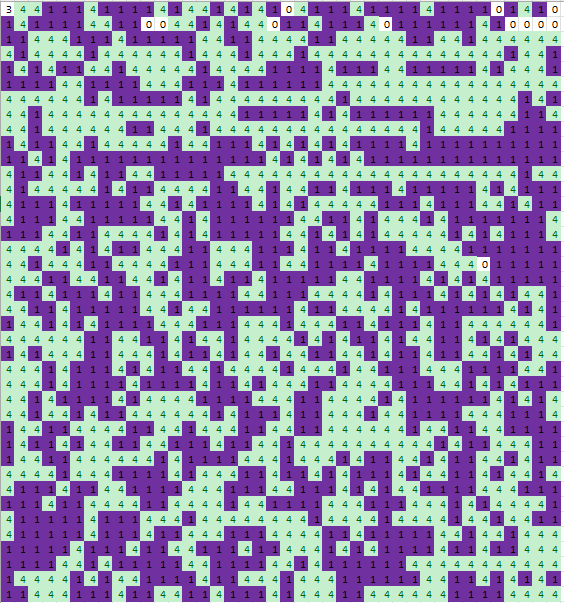
\includegraphics[width=\linewidth]{peacefull coexistance.png}
		\caption{}
		\label{fig:frenchriot}
	\end{figure}
	
	\subsection{Ethnic Cleansing}
	initial conditions: C = 0, Q = 560 purple and 560 green, v = 2, T = 0.1, L = 0.8\\
	\\
		\begin{figure}[H]
		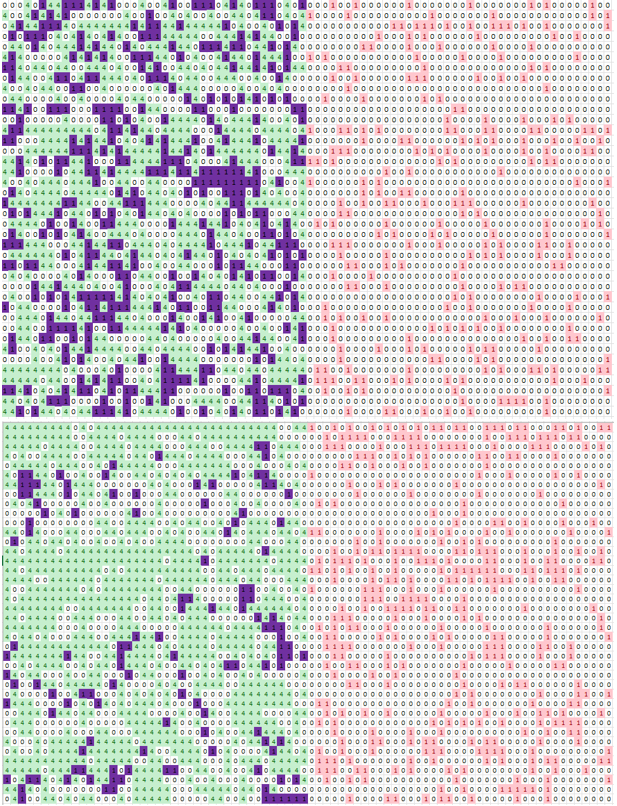
\includegraphics[width=\linewidth]{ethnic_cleanse1.png}
		\caption{}
		\label{fig:frenchriot}
	\end{figure}

\begin{figure}[H]
	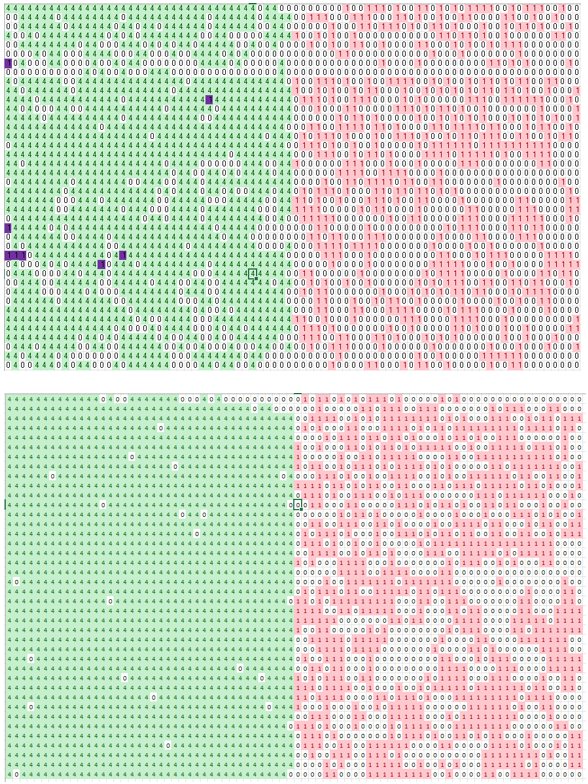
\includegraphics[width=\linewidth]{ethnic_cleanse5.png}
	\caption{}
	\label{fig:frenchriot}
\end{figure}
from the above images we can see our green group from the model multiplying over 30 iterations and slowly removing all of the purple group. Over a long period of time (30 iterations) we always see one group completely get rid of the other group.\\
\\
This can be compared to "competitive exclusion" which is the idea of two species being in a confined space both competing for resources and in the end one species may get rid of the other taking all the space for its own expansion and more resources. However when a predator is introduced to regulate the growth of the species then both can end up surviving for a longer period of time.

\subsection{Effect of Police Density on Extinction Times}
Police in my model can be seen as predators, they themselves can not be taken away by the prey (ethnic groups) however they themselves can take them off the board, even if it is a short period of time. This in turn helps keep the ethnic groups alive for longer than what they usually would be, However their coexistence is not peaceful. Both groups are still taking each other off the board and rioting. \\
\\
In order to see the effect that police have on the length of time that the groups can exist together without wiping each other out I run the grid changing the density of police on the grid starting out with 0 P's on the board and moving up to 150 adding 3 each time. The model also runs 50 times at each P density. This gives figure 21


\begin{figure}[H]
	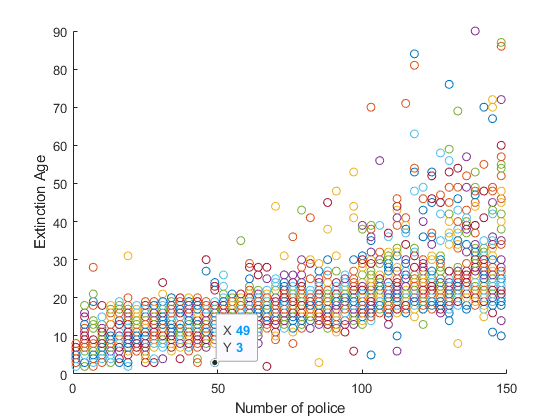
\includegraphics[width=\linewidth]{Extintion Age vs Police Density.png}
	\caption{}
	\label{fig:frenchriot}
\end{figure}
We can see a trend in this graph, it is clear that as we increase the density of P's on the grid that the length of time our ethnic groups live for increases. Further more if we find the average extinction time for each density we get figure 22


\begin{figure}[H]
	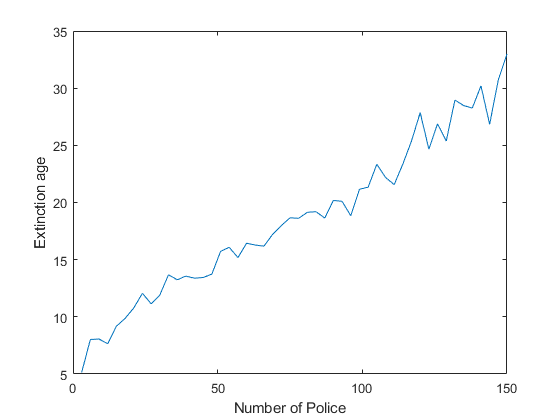
\includegraphics[width=\linewidth]{Extintion Age vs Police Density 150.png}
	\caption{}
	\label{fig:frenchriot}
\end{figure}

This makes it very clear that there is a linear relationship between cop density and extinction time as we see the extinction age increasing from beginning to end.

	
	\section{Model 2 Evaluation}
	With a high legitimacy L=0.9 two ethnic groups live together peacefully in my model, but when this legitimacy is reduced to L = 0.8 we observe ethnic cleansing take place. The addition of police can help prolong the length of time two ethnic groups live together before one wipes the other out and adding more police increases this time even more however it seemed that ethnic cleansing still took place even with very high cop density's
	\newpage
	
	\section{Conclusions}
	Agent based models may not be quite as complex as an actual riot or a revolution. However studying them can Help us understand what variables may effect a revolution and how smoke can be used to bring a riot to a quick end.
	
	
	
	
	\bibliography{abm}
	
	
	
	
	\newpage
	\section{Appendices (Matlab Code)}
	\lstset{language=Matlab,%
		%basicstyle=\color{red},
		breaklines=true,%
		morekeywords={matlab2tikz},
		keywordstyle=\color{blue},%
		morekeywords=[2]{1}, keywordstyle=[2]{\color{black}},
		identifierstyle=\color{black},%
		stringstyle=\color{mylilas},
		commentstyle=\color{mygreen},%
		showstringspaces=false,%without this there will be a symbol in the places where there is a space
		numbers=left,%
		numberstyle={\tiny \color{black}},% size of the numbers
		numbersep=9pt, % this defines how far the numbers are from the text
		emph=[1]{for,end,break},emphstyle=[1]\color{red}, %some words to emphasise
		%emph=[2]{word1,word2}, emphstyle=[2]{style},    
	}
	
	
	
	here is my code for my riot simulation
	\lstinputlisting{civil_violence_model.m}
	here is the code for my jail
	\lstinputlisting{update_jail.m}
	
	







\end{document}